\documentclass[10pt,twocolumn]{article}

% use the oxycomps style file
\usepackage{oxycomps}

% usage: \fixme[comments describing issue]{text to be fixed}
% define \fixme as not doing anything special
\newcommand{\fixme}[2][]{#2}
% overwrite it so it shows up as red
\renewcommand{\fixme}[2][]{\textcolor{red}{#2}}
% overwrite it again so related text shows as footnotes
%\renewcommand{\fixme}[2][]{\textcolor{red}{#2\footnote{#1}}}

% read references.bib for the bibtex data
\bibliography{references}

% include metadata in the generated pdf file
\pdfinfo{
    /Title (The Occidental Computer Science Comprehensive Project: Goals, Timeline, Format, and Advice)
    /Author (Justin Li)
}

% set the title and author information
\title{Reading Spectrograms}
\author{Nathaniel Hogan}
\affiliation{Occidental College}
\email{nhogan@oxy.edu}

\begin{document}

\maketitle

\section{Problem Statement}

The problem that is being worked on in this project is the challenge of phonetic transcription. This project answers the question of whether or not a Neural Network can read and transcribe sound through the medium of spectrograms. More specifically, this project attempts to measure and explain the aspects of English that are more easily identified by the specific Neural Network that I used, as well as identify the things that the model does well compared to what a human can see. An extension to these theoretical questions is whether, if a model can predict sounds, can an algorithm be used to turn individual sound-based classification into broader utterance recognition using repeated guesses. 

The reason why phonetic transcription is important is because it is an important step in the preservation of endangered languages \cite{LanguageDeath}. If it worked perfectly and without flaws, a system like this could be used by linguists to expedite the process of analyzing languages, which would allow them to spend more time collecting data in the field.

\section{Technical Background}

An important thing to understand for this project is what a spectrogram is and how it works. A spectrogram is one of the ways to visualize sound in general and is one of the two primary visualizations that linguists use for human speech. Spectrograms are particularly useful because they show three variables in one place. It is a representation of the frequency on the y axis, time on the x axis, and amplitude (how loud the specific frequency is at the given time) as either the darkness or the color (depending on implementation of the spectrogram). Figure 1 shows the spectrogram feature that the linguistic program Praat generates from wav files. Praat also shows the waveform which only shows amplitude vs. time, excluding the extremely important aspect of frequency, which is used in the distinction of sounds. 

Additionally, the reader needs to understand the basics of how Neural Networks work. Essentially, in the context of images, different aspects of an input image are analyzed with different nodes in a hidden layer, for which the importance of said connection is stored using a weight \cite{NeuralNetworks}. This means that as training occurs, these weights are modified to more accurately predict the correct classification. The input is the size of the image, the output is the number of classifications for the problem, and the number of hidden layers can change. These weights act as a function, turning the input into the output, which means that you can perform calculus functions on it if needed for optimization. 

\begin{figure}
    \centering
    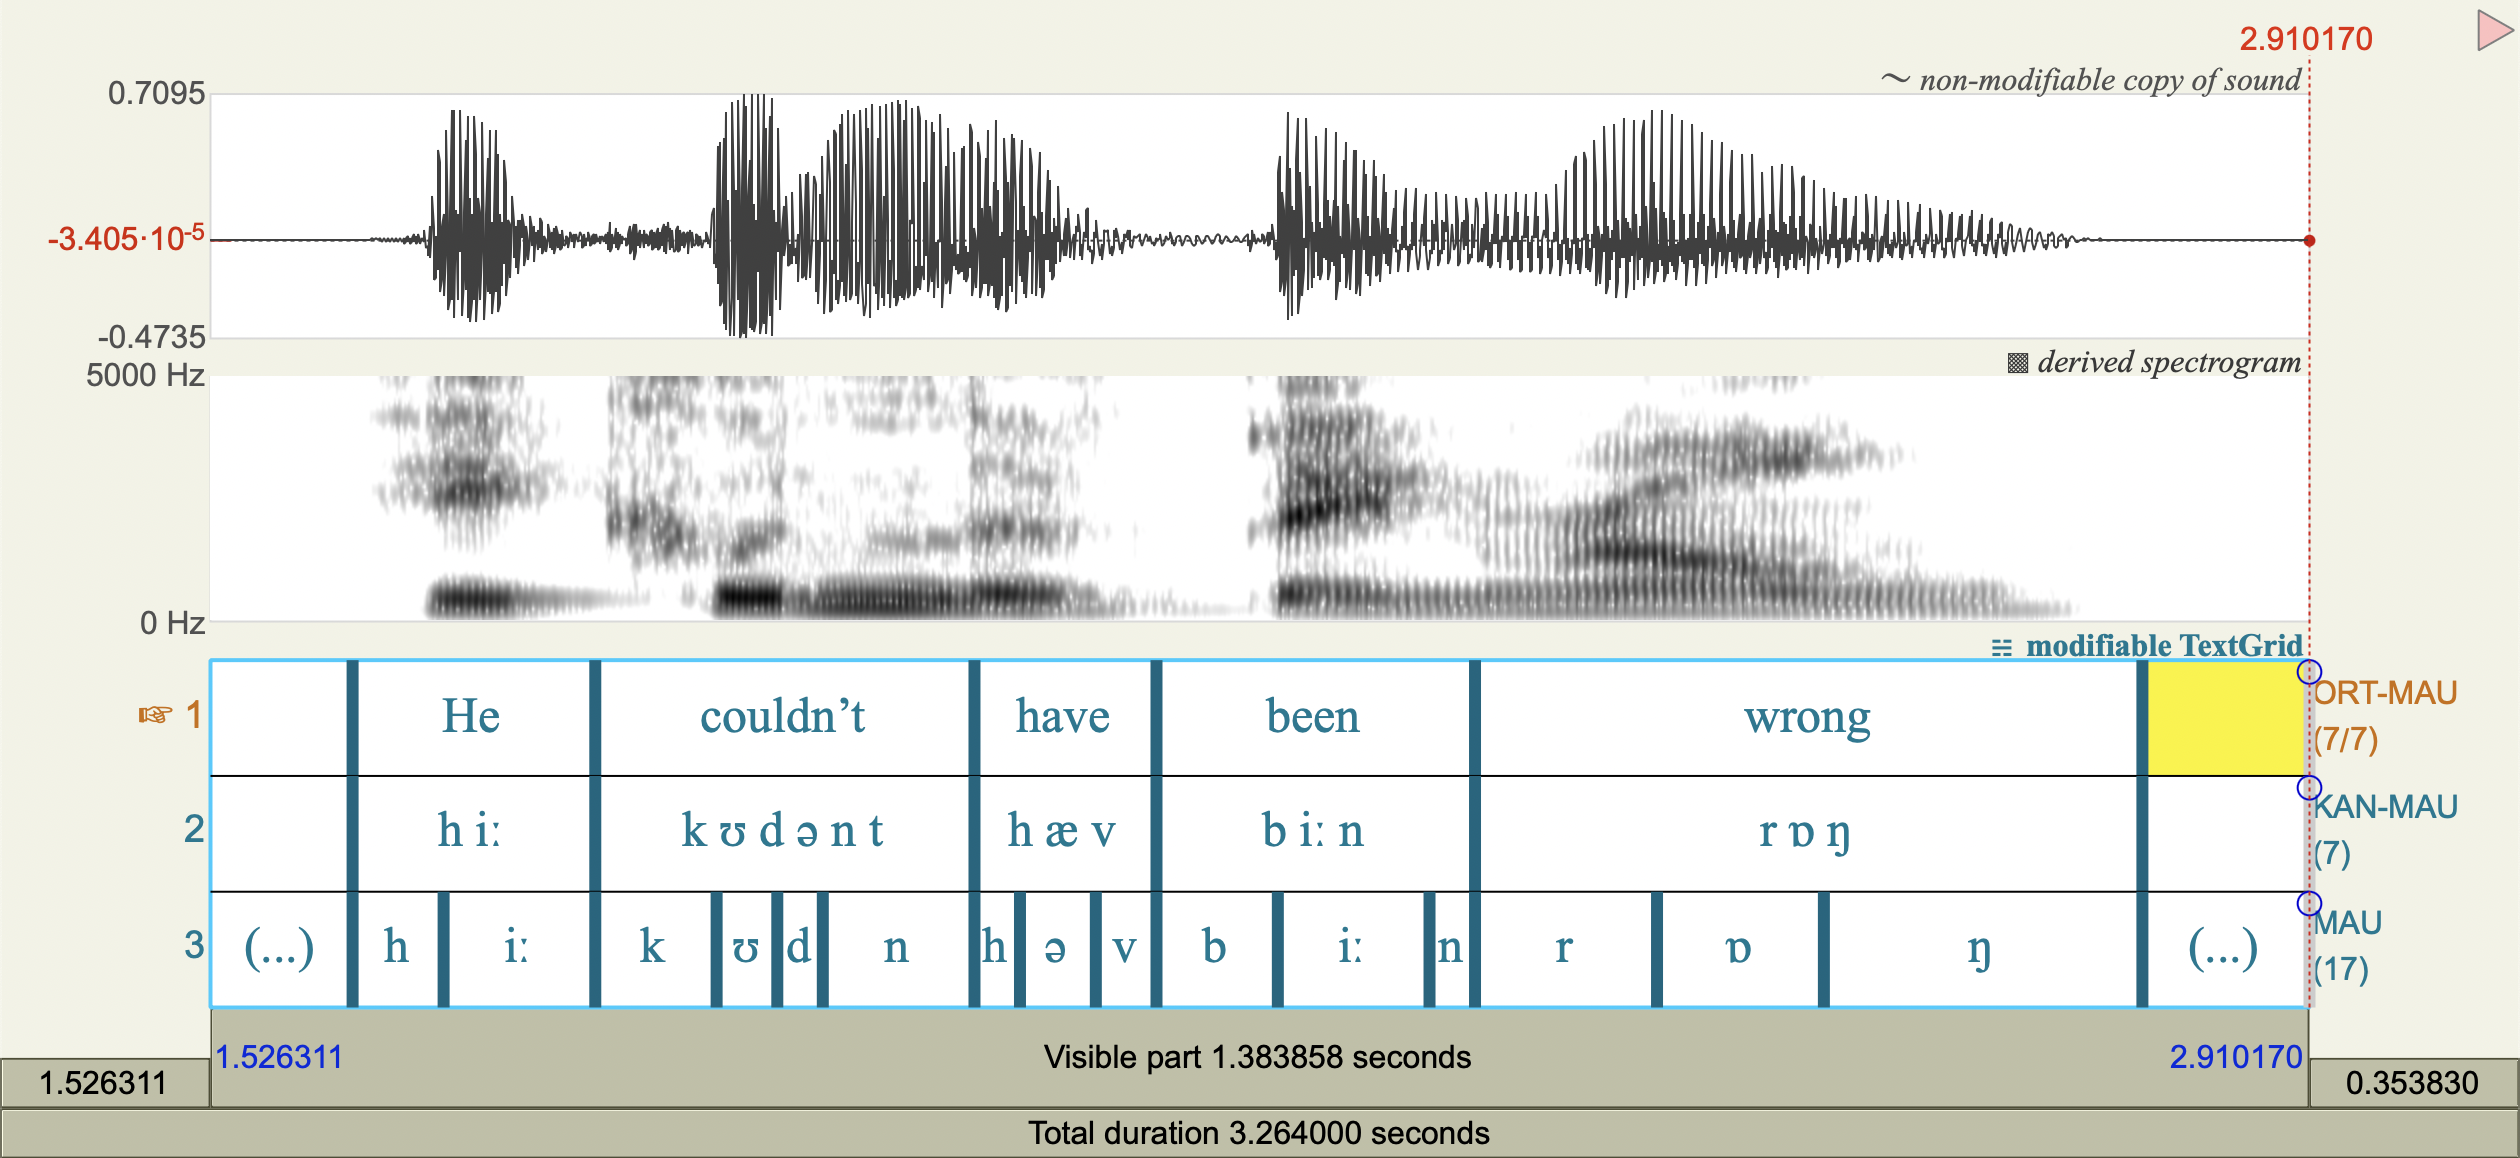
\includegraphics[width=.95\linewidth]{spectrogram.png}
    \caption{
        An example of a spectrogram.
    }
    \label{fig:first-page}
\end{figure}

Figure 1 shows the spectrogram for one of the speakers saying “he couldn’t have been wrong.” The dictionary transcription is shown in the second tier. The third tier shows the individual segmentation, which is dynamic and looks at aspects of the spectrogram in order to properly place these segmentations. If you notice the transcription for “couldn’t” has the upside down e that is called a schwa. This sound is actually not present in the audio file and instead the n is syllabic, so it can act as its own syllable. Additionally, the t is unreleased, meaning that it does not show up in the spectrogram. The sounds are not shown as unreleased or syllabic (and the vowels are not shown as nasal when they should be in a few cases), which is fine for the context of this project (and easier since all n’s will look the same to the praat script), however it is missing some context that a human segmented sound would have.

\begin{figure}
    \centering
    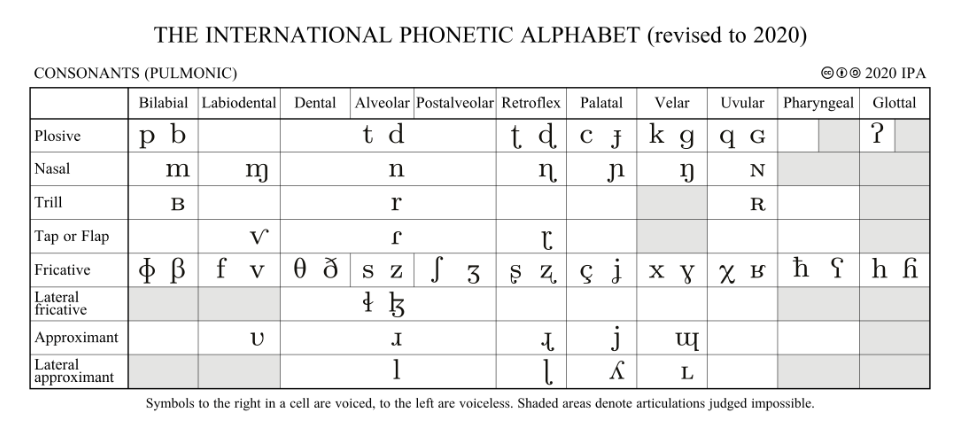
\includegraphics[width=.95\linewidth]{consonant.png}
    \caption{
        IPA chart for consonants.
    }
    \label{fig:first-page}
\end{figure}

\begin{figure}
    \centering
    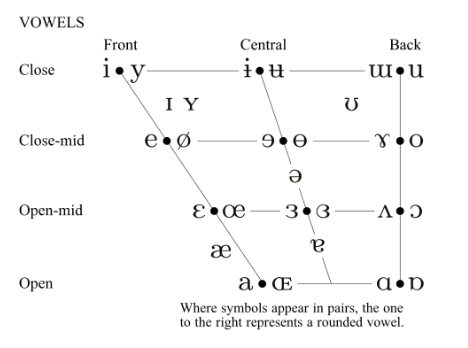
\includegraphics[width=.95\linewidth]{vowel.png}
    \caption{
        IPA chart for vowels.
    }
    \label{fig:first-page}
\end{figure}

Figures 2 and 3 show the IPA chart, which is the standard way of representing sound according to the International Phonetic Alphabet association. There are two different charts, one representing vowels and one representing consonants. The vowel chart represents where your tongue is when producing the sound, with left being front and right being back. Similarly, for consonants, the farther to the left, the closer to the front of your mouth that place of articulation is.


\section{Prior Work}

Image recognition, more specifically image classification is a large part of what this project is attempting to accomplish. Image classification is second nature to humans but more challenging for computers. This project differs slightly from work in generic image classification fields because the images that are being classified are not as easy for non-trained humans to distinguish. This leaves room for a neural network to perform better than humans potentially, as well as it makes it harder for features descriptors to be used for the classifier. This method of using specific features was overshadowed by deep learning models that use non-linear information processing. One paper suggests CNNs as the major architecture for image recognition \cite{CNN}. This type of model creates convolutional and pooling layers which alternate. The convolutional layers act as feature extractors while the pooling layers help to alleviate distortions and translations in the input. This style of model is not exactly what I am using, however it gives an idea of the different methods for neural networks.

Very recently a paper was published online (it had existed offline for about a year) that analyzed the ways in which Neural Networks (more specifically deep neural networks) were able to train speech recognition models \cite{SpectrogramML}. This paper includes a lot of discussions of both machine learning and spectrograms which are similar to what my paper will do. This paper focused more on vowel classification and voiced vs. unvoiced sounds than my project did (which synergises with this project because one of the struggles of my model was vowel recognition). One important takeaway from this paper is the idea that when a linguist looks at a spectrogram they are using their prior knowledge of the way spectrograms look in order to focus on the distinguishing parts. Models that are not trained with this in mind might not put enough emphasis on these important parts which could lead to unoptimized training which would hurt the accuracy of certain models.

Another similar paper to this project created a model that can turn an audio into the international phonetic alphabet \cite{UniversalIPA}. They mentioned the lack of quality audio with close transcriptions that are available, so they took automatically aligned data and manually verified that the segmentation was good enough. They used a pre-trained model and fine-tuned it to predict IPA. One interesting thing from their work is that when predicting IPA in a language that was not included in their training data, their model with fewer samples performed better. This could mean that for my model, if tests are done on new languages, that more data for training is not necessarily better.

These two papers influenced my project the most since their topics are extremely similar to what I am doing and have takeaways that either validate the work that I did (such as the quality of data in this specific area being poor), or shape the way that I attempted the problem. 


\section{Methods}

This project has three main aspects, those being the dataset, the neural network, and the algorithm that turns many single sound guesses into a series of predictions for a word or utterance. 


Finding/creating the right dataset is extremely important in a project such as this because it is what the model is going to be trained on, meaning that a bad dataset can cause problems later on and that fixing problems with it after the models are trained becomes problematic. It was decided to use English as a starting language and other languages and their sounds could be added if time permitted or as an extension to the project. The model would still be able to make predictions about similar sounds in other languages without explicit training where the model would act as a pre-trained model. 

Training different and new models for different purposes is undesirable due to the time it takes. One solution is to start with a pre-trained model and use it to transfer knowledge from one language to another, which would be adding more information from other languages or speakers for the continuation of this project \cite{PreTrained}. Any model created by the neural network is expandable. The exact subset of the data used is common voice file 110116 to file 150128, meaning that the inclusion of more of the English dataset or the inclusion of the other languages would be simple to perform given data already downloaded. 



	
Models exclusively trained on English may struggle with context and production differences between languages that are visible in a spectrogram, however this difference also might make the dataset harder to understand if a multilingual set of data was chosen. Different languages have different contexts for sounds and produce similar ones slightly differently. This project starts with English as its base language, however the ability to expand into other languages is possible.

Ideally, there would already exist a dataset of English sounds, however the best that was able to be found was the “first phoneme based speech dataset in the entire world” in Persian \cite{PCVC}, which was not within the scope of my project. Instead, a dataset that had English (along with other unused but potentially useful languages) was selected. There are many datasets that contain some phrase and its phonetic transcription, however in order to create a dataset of sounds, the timing of each phoneme is particularly important, and the dataset chosen provided this segmentation of the sounds. This segmentation was provided using a forced aligner, meaning that it provides a solid but imperfect segmentation of the data. Forced aligners use programmed dictionaries, which use a triphone acoustic model capable of looking at clusters of phonemes, which increases the accuracy of the aligning given the context of each sound, to mark the beginning and end of each sound \cite{ForcedAligner}. Forced aligners fail to deal with the stress at the sentence level, which often will affect the reduction of vowels, which could lead to proper phonemic transcription (the right intent from the speaker) but improper phonetic transcription, which is what this project cares primarily about.



This dataset uses a neutral emotion for all speakers which helps to avoid some variation within the same sound, which would cause issues with the training of the model \cite{Emotion}. This also means that the model might struggle to understand the voice of someone showing emotion.

The dataset is in the form of .wav files and .TextGrid files, a file format specific to Praat, the most popular program used for linguistic analysis. This TextGrid has 3 tiers all created by the forced aligner which contain the word, its phonetic dictionary entry, and the individual sounds segmented. This third tier is all that matters for the scope of this project. Initially, a script written by Katherine Crosswhite using the Praat scripting language was used to extract desired sounds and convert them into their own individual wav file. This script outputs a .Sound file by default, and had to be modified to output as a .wav file in order for the rest of the process to work. 

An example of the spectrogram and TextGrid alignment is shown in figure 1 in the technical background section.


Only a subset of the data was used. The total dataset (including other languages) is over 116 hours long, and English is the largest dataset. A total of 2061 sounds make up the dataset used in this project. These sounds come from 264 utterances within the Common Phone dataset. Specifically it is utterance 110116 to utterance 150128, where multiple sounds are permitted to come from the same recording.

It was decided to not select only the best examples for each sound in order to preserve the diversity of the dataset. Both to see if the model can learn given non-perfect data as well as to make it as expandable and simple to produce as possible. The model will be good at identifying sounds in the perfect scenario with cherry picked sounds examples, but a good model will be able to maintain accuracy even when the training data is imperfect, as well as imperfect data will train the model for imperfect testing data in a better way.

    
There were some issues with the quality of the exported .wav file so this script was modified again to write into a file the start and end times for each specific sound and a python program using the AudioSegment library segments the sounds instead. 
	
A python program was then used to create a spectrogram from the segmented .wav files, which concludes the creation of the images for the dataset.



The model was trained using the nn library within pytorch. Python was going to be used regardless because of the ease of use and the fact that it is used in the processing of the dataset, but there were a few options for the specific library to be used for this project, such as TensorFlow. One reason why pytorch was chosen is because it is used in a Forced Aligner that I am familiar with, as well as the fact that some of the aspects of TensorFlow that make it better for larger scale projects are not as useful for the scale of project that is being worked on. Additionally, the ease of use for pytorch makes it so that more effort can be put into other aspects of the project that are also important. 

The neural network uses a standard gradient descent (SGD) optimization algorithm which calculates the gradient of the state of the layers and uses it to find the change that would minimize the function’s loss, which will improve the model as much as it can. The training algorithm turns the input image into a 128x128 image with color (3 color variables per pixel), which means that the input layer is 49,152 nodes. The output layer is the number of sounds included, which is 16 for the most developed model so far. There are 3 hidden layers with decreasing amounts of nodes in each. It contains layers with 2048, 2048, and 512 nodes. The inclusion of more hidden layers did not provide a meaningful difference in performance so it is possible that these layers are already partially redundant.

A standard neural network was chosen instead of a CNN or other model because this style of image recognition is not identifying something that is part of the image, it is recognizing the image as a whole, meaning that the convolutional layers are less useful.

Many models were trained using different variables in order to determine the optimal settings for the neural network. Other optimizers were also looked at, with Adam being a possible choice. SGD was chosen because Adam has a dynamic learning rate that can sometimes fail to find the optimal local minimum. At the scale of this project (and from the minor testing using both optimizers) there was no meaningful difference between the two.

A total of 100 epochs were used in the project due to limited resources. There was a downward trend in the change at each epoch, with the first epoch with 40\% accuracy was epoch number 51, meaning that the network spent the last 50 or so epochs making the model more consistent rather than hitting a new high percentage. Presumably given more time (and the flexibility to use a lower learning rate), the model could perform better than it currently does.

The last part of the project is a collection of smaller algorithms that work together to create a rolling window that allows the model to make multiple predictions in a row which, when put together, approximate a prediction of the whole utterance. This is done using the AudioSegment library to create the segments of audio needed for the window. It was chosen to use 200ms for each slice of the rolling window with a 50\% overlap in between slices. 



Sounds were added in small batches with the model updated (retrained) for each new set of sounds. This was done to make sure that the model is working as expected at every step of the way. Often similar sounds were added together since those sounds would be the most challenging for the model to tell apart (such as voiced and voiceless pairs being added together). The amount of data per sound was determined by the dataset, every existence of each sound was used so more common sounds had more data included, for example there were 149 “m” sounds but 210 “n” sounds. The first 10 examples of each sound were chosen to be in the testing dataset. Typically the data is split 80-20 or something similar, however I decided to have the same amount of testing data for each sound.

The total sounds used were the diphthongs ai and ei, the vowels e, æ (called ash), schwa, and consonants d, f, g, k, m, n, s, sh, t, v, and z. These sounds are representative of many different aspects of English sounds, although it is not complete.


\section{Evaluation Metrics}

After being trained, the model is tested using the test data set consisting of the first 10 instances of each sound. This style of testing is black and white, testing whether the model made a correct guess or incorrect guess. This style of testing is lacking a lot of context since similar sounds usually look similar in terms of the spectrogram, meaning that it is possible for the model to make a good guess that is only slightly incorrect, but it is being graded as though it got it 100\% incorrect. 

The literature mentions that the different formants (prominent frequencies) have physical differences, and that since your mouth shape is a gradient, similar sounds will have similar characteristics. This means that distance metrics are possible to create, it is just unknown how to quantify the distance \cite{InterpretationOfSpectrograms}. 

Two distance metrics were created, one for vowels and one for consonants. Closeness is measured from zero to ten with a lower score being better. For vowels, the International Phonetic Alphabet vowel chart is reduced into a 3 by 4 chart and the euclidean distance is calculated between individual points on this chart. For consonants, for any guess that is in the right column or row, a distance is provided depending on how many boxes of separation are between the guess and correct answer. If the guess was not in the right column or row, a distance of 10 was provided since the guess was not good enough. A distance of 10 is also given if the model predicts a vowel for a consonant and vice versa. These distance metrics allow for a more nuanced interpretation of the model's accuracy and they give more insight into what the model is particularly good or bad at. 

Columns in the IPA consonant chart show similar places of articulation but with the incorrect manner. This means that the model may have seen something that it recognizes, but made the incorrect guess. It is hard to determine how much to penalize a guess such as this since the different manner types are not different from each other in an ordered way. This project left them as 10, however it may work to place them somewhere on the scale from 0 to 10, such as 5. The literature is unhelpful in this department.


For the purposes of this project, a distance of zero was provided to consonants that were within the same box, which means voicing was ignored when measuring the average distance. This was done because the penalty for getting the correct articulation but missing a small detail that points out voicing should not be very high. Voicing should not affect the shape of the spectrogram besides a darker bar at the bottom, meaning that the model predicting the other voicing is making a great guess given the majority of the image.

\section{Results and Discussion}

An analysis of the results demonstrates that the answer to the question ‘Can a Neural Network read a spectrogram’ is yes. The results for this project were promising but not perfect. An analysis of the results can also give some insight into which aspects of spectrograms are easier or harder for this style of model to understand. The accuracy of the model is the most important result, since regardless of whether or not the rolling window algorithm works, if the model is making poor predictions, then it is not as useful. 

The most current results are that the model has a 39.4\% accuracy with an average distance of 3.23. The number that it gets correct (63/160) is more than the number for which the distance is 10 (40/160) which is a good sign that the model is working correctly. A model that was randomly guessing should have an accuracy of 6.25\% for the given data. 

Since the model only has a 39.4\% accuracy given ideal conditions, it is no surprise that the rolling window results were poor. A few of the predictions were close, however only 2 out of the 30 slices were correctly predicted. 


The biggest obstacle in terms of the model was memory. A result of about 40\% is okay for this project, however increasing certain variables too much crashed the MacBook used to perform the training. Specifically, having too many nodes in the neural network’s hidden layers caused issues, as well as running too many epochs. It is for these reasons that the training was done carefully and not to excess, although the time in which the crash occurred, the current prediction for the model exceeded what was previously possible, meaning that this project is not particularly near its optimization, that there is room to develop it more.


The models created are very good at identifying vowels as distinct from consonants, however it is not very good at distinguishing between vowels. One reason for this is that, as mentioned above, vowels in English can have overlap in some of the frequencies and often require the context of the word to understand. Additionally since syllables are often in the form of consonants surrounding a vowel, it is more likely that adjacent consonants will modify the vowel sound than the other way around. A language with less overlap in vowel space would be easier for this model to distinguish. 

\begin{figure}
    \centering
    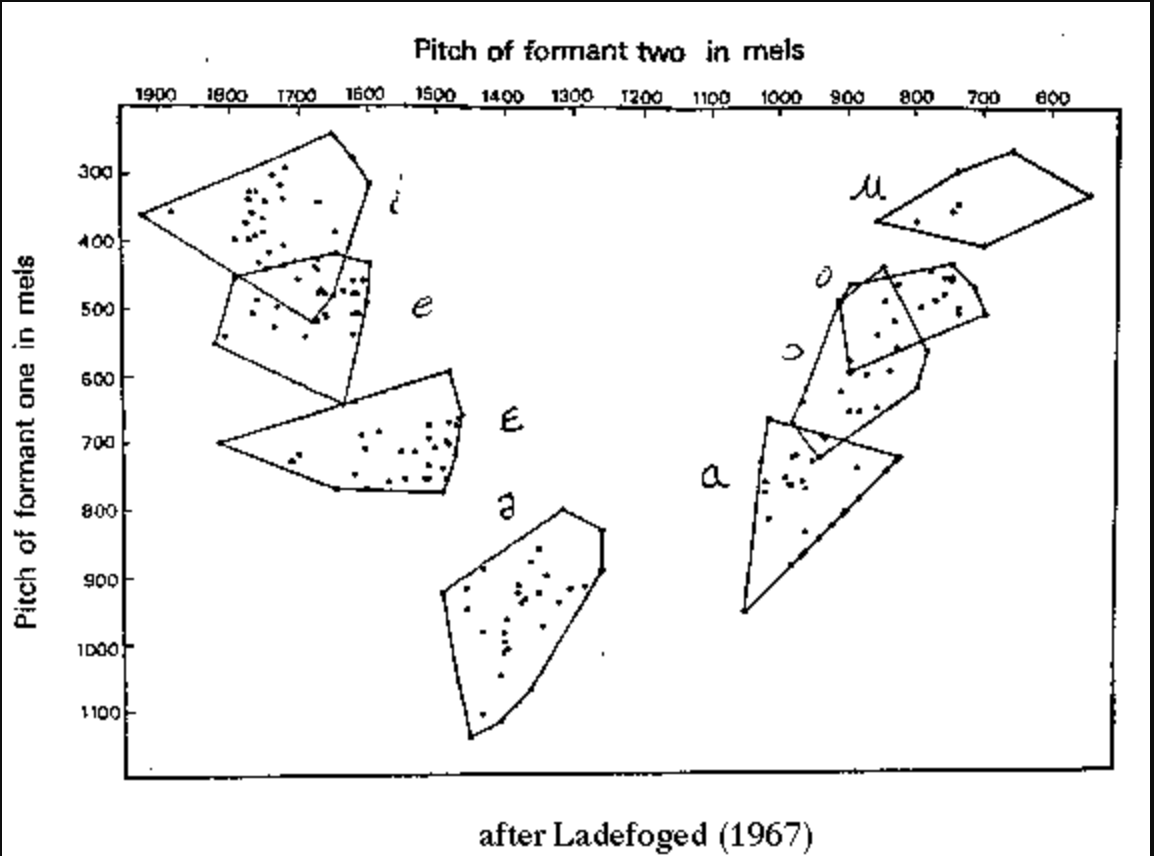
\includegraphics[width=.95\linewidth]{vowel_space.png}
    \caption{
        Example of a vowel space.
    }
    \label{fig:first-page}
\end{figure}

Figure 4 shows an example of a vowel space, which shows the area within the mouth (and within the chart) that is understandable to humans as whichever vowel. There is some overlap and some areas with no vowels present. The vowel space for full English is more complex, having more vowels and more overlap, and depends on dialect.


The model struggled less with the schwa sound and more with the ash sound, with about half accuracy on the other vowel sounds used. The two diphthongs used in the training data were predictably easy for the model to understand because of the movement in the frequencies that are unique to those sounds. 
For consonants, the model struggled most with the k sound and the v/f sound. It makes sense that the model might struggle with the plosive sounds (the sounds that stop air before releasing it) because much of the spectrogram is actually the absence of anything, which could be any of the stops, not just whichever one the spectrogram represents. This is why we see a large amount of t and d guesses for the sound k. The model being bad at understanding the v and f sounds makes less sense to me. They look like an z or s in the fact it should be very chaotic without many specific patterns in the frequencies. If the model struggled as well with the z sound it would make more sense, but for some reason the distinction between these chaotic sounds is enough to make z, s, and sh all easy for the model to understand, but not for v or f.



The model was extremely good at identifying the nasal sounds n and m. This makes a lot of sense because their form is more vowel-like since they have a larger cavity for the sound to bounce off of (your nose). There were only 3 predictions in the testing dataset that incorrectly predicted that a nasal was a non-nasal. Between the nasals there was a small amount of confusion, with n being predicted for many of the m sounds, but one reason for this could have been that the dataset has more n examples than m ones. 

The models were surprisingly poor at determining the voicing of consonants. Voicing is visible in a spectrogram as an obvious bar at the bottom and is often the first thing that a linguist will look at in a spectrogram. This quality is particularly useful for ruling out certain sounds because it removes half of the possible options for consonants. I believe that, given enough training time, this pattern would be understood, but the way that the models were trained they do not get feedback about nor do they have an understanding of the different classes that each sound belongs to. They look at each sound as distinct from every other one and not as part of a system. 



Figure 5 shows the type of spectrogram that the model will look at for training and testing data. The sound is an “s” sound, and you can see the chaos in the top, there are no clear lines present due to the way the sound is produced in the mouth. 

Figure 6 shows the spectrogram for the sound “z” which is the voiced equivalent of s. You can clearly see the darker band at the bottom called the voicing bar, which basically shows that the sound is voiced. 


\begin{figure}
    \centering
    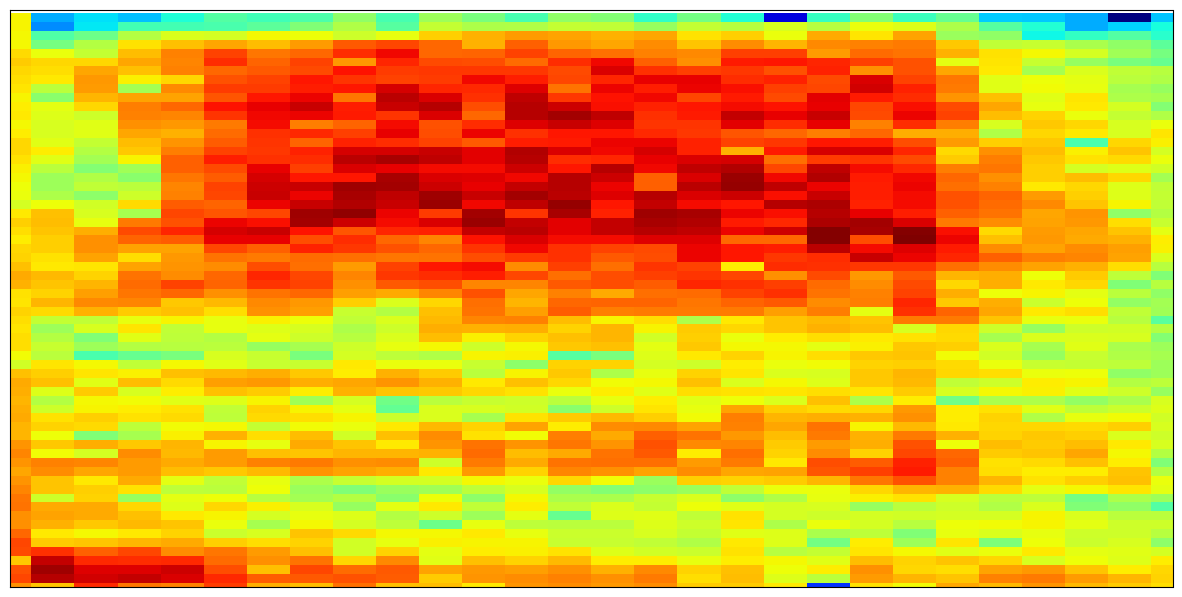
\includegraphics[width=.95\linewidth]{s_sound.png}
    \caption{
        An "s" sound.
    }
    \label{fig:first-page}
\end{figure}

\begin{figure}
    \centering
    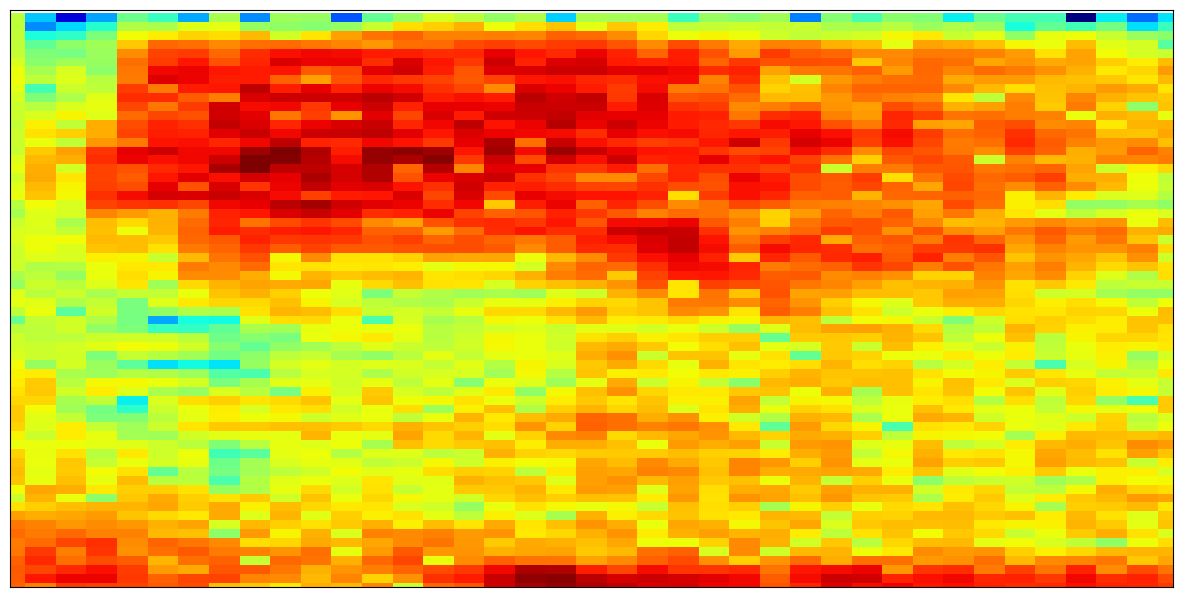
\includegraphics[width=.95\linewidth]{z_sound.png}
    \caption{
        A "z" sound.
    }
    \label{fig:first-page}
\end{figure}


To a human, the difference between these two is clear if you know what you are looking for, and the model is more right than it is wrong predicting between these two sounds, however there are 3/10 incorrect guesses of “s” for z in the testing dataset and 2/10 incorrect guesses of “z” for s.


As mentioned in the methods section, there were originally some issues with the quality of the spectrograms for shorter audio files. Switching the method of creating these wav files helped, however they were not as clear as would have been expected. The issue partially comes from the code that creates the spectrogram. It outputs the spectrogram in a similar image ratio, regardless of the length of the sound. This means that if the utterance is more than a few seconds, the spectrogram includes up to 5000 hz of frequencies, which is more than enough for understanding human speech. The issue is that when these utterances are split into individual sounds, the program wants to keep a horizontal style of image, so it compresses the spectrogram. If this were done similarly for each sound, there should be little issue since we would just be redefining what the model is reading, however since certain sounds are shorter or longer than others, the same sound can look slightly different in the spectrographic representation. A nonlinear model should be able to work through these problems assuming that the training data is all correct, but given the training possible, there is the possibility that this affected the accuracy of the model. 



The dataset was segmented using a forced aligner and although forced aligners are a great start, it is hard to beat human-segmented data. Occasionally the same sound will look different in the spectrogram, which would throw off the model.




There is a trade off between diversity and consistency within the context of this project. Having an extremely phonetically similar dataset would increase the accuracy of the model, however there are obvious ethical problems with excluding any group of people in specific. Beyond different dialects that may or may not correspond to race or some other characteristic, sex, gender, gender identity and expression also have acoustic effects on speech, which is visible in the spectrographic representation \cite{PhoneticsSexGender}. The dataset only provides information about gender, age, locale, and accent. Given this information it can be confirmed that this set of data is very diverse with a skew towards speakers having a United States accent, a perfect gender balance, and a good variety of ages from teens to eighties. 

The amount of data plays a role in the final results of the model. Using a small subset of the total Common Phone dataset increased the consistency of the training dataset, however it provides less opportunity for different styles of voice. Only 264 different speakers were used, and although the demographics were different between speakers, it could have been better, using more accents and different locations for speakers. A good extension to this project would be to use more data to improve the models. The model may not improve in terms of pure accuracy with more data, however it will become more aware of the differences between the speech of different people. Training on the other languages provided in the Common Phone dataset would also be an easy extension given the work done.


English is a very complex and dense language phonetically, using more sounds than some languages, which means that there are perceivable differences between some sounds that another language might not have. A language with fewer and more consistent pronunciation would probably have been better if the goal was to specifically target one language, however if language is to be generally ignored and the sounds themselves prioritized, more training data and time would be more useful. 



	

I am unsure of how to encourage a model to understand particular aspects of a sound, but I wonder if a subset based model would work well. Give overlapping datasets representing place and manner of articulation and voice quality and have the model make three guesses for each sound, triangulating the correct sound and understanding the relationships that led to each guess.

There is not very much prior work done on specific distance metrics for sounds, so the metrics created for this project do not have much of a literature basis. The distances are logically sound, but the extent of the distances was created more arbitrarily meaning that more research would be necessary to determine the quality of this set of distance metrics. These metrics also are attempting to compare the distance between sounds including the three subcategories mentioned above, being place and manner of articulation and presence of voicing. The literature does not provide a weighting for which aspect is most important, which is especially challenging because each aspect has a different scale on which it can be graded. The vowel metrics should be more accurate because voicing is not a problem since vowels are characteristically voiced. 

The default distance for two sounds that are not similar being ten was also arbitrary and causes some problems with the interpretation of these metrics, especially with the average distance. The average distance being skewed towards ten means that an average distance of 3.2 is not as bad as it looks, but without looking at the specific predictions it is hard to know exactly what this number means. 

\section{Ethical Considerations}

There is not much technologically that can be abused with this project. Machine learning can take a lot of processing power, so if this project were expanded using more powerful machines, it is important to pay attention to the pollution created from the energy used. 

Most of the ethical considerations come from societal uses. The bias within the dataset was mentioned in the discussion section. Any bias in the dataset will be visible if this method of reading spectrograms is applied to anything. Models trained on incomplete data (in this case missing any sound possible) will be missing the ability to make good predictions if presented with that data. This is called negative bias, where the model is missing the available classes to properly label certain sounds \cite{DatasetBias}. 

One aspect that could be continued from this model is not only identifying sounds, but identifying the way people make these sounds. If a model similar to this one were to attempt to categorize speakers based on race or gender or sexuality based simply on how they talk, something like this could potentially profile people. A spectrogram reading model would be much worse at profiling people than a human is for a long time, however we must consider the widespread applicability of a machine that is able to do this. In terms of profiling, something that only looks at individual sounds would also be much worse than something that looks at multiple sounds in a row since a lot of information can be obtained from the context surrounding sounds, not particularly the sounds themselves. This technology also already exists in a more competent manner than you could get from a spectrogram \cite{Profiling}.

One reason to create a system like this is to help global inequity. Thousands of languages are dying out due to globalism, and linguists can use a tool such as this to quicken the process of recording these languages. Something like this has the capability to help store the language and culture of peoples for whom it may be lost in the next 10-100 years. There is a whole other argument about the ethics of protecting the language of another group that is explained well in a book by David Crystal about Language Death \cite{LanguageDeath}.

\section{Replication Instructions}

First download python (I used version 3.9.13) and Praat (I used version 6.4.05). Download the Common Phone dataset \cite{CommonPhone} and prepare a folder within the dataset that combines both the wav files and the TextGrid files. Also prepare a separate folder to house the modified dataset used in this project. A folder titled data with a testing and training dataset in individual folders is used, with folders containing each sound within both. 
	
Open Praat and select open, choosing the get\_timestamps.praat in the github. Change the file so that the correct sound is selected at the top and the path to the file which stores the timestamp data to be wherever your file is. Once this runs, you should see a text file containing all of the information to create our wav files and spectrograms. Open split\_from\_txt.py and modify the directories to match whatever you are using. Then run the file and you should see a collection of wav files wherever you want them. Then modify spectrogram.py to have the right input and output locations. Then run it and you should see a collection of png files that are spectrograms. If they are not already in the training or testing folder then place them there, moving the first 10 into testing. Once this is done for every sound desired, then you can prepare the file neuralNetwork.py. Make sure that the datasets are the right directory, then run the file and the model should start training. 


\section{Code Architecture Review}

The code is organized into a collection of programs that mostly do small things to data, with one large program that does all of the training once the dataset is created. It makes sense to separate the dataset creation and the neural network code because the dataset is created in multiple instances while the model is only trained once. The other files are kept separate partially because multiple languages are used (python and praat), as well as the fact that verifying that things worked correctly at every step saved a lot of time when creating the dataset for the first time, as well as making sure that each sound does, in fact, sound as it should. As mentioned in the replication instructions section, there is a praat file (get\_timestamps.praat) that writes a text file containing all of the timestamps for whichever sound is being added. Then a python file (split\_from\_text.py) is used to read this file and segment the sound. Then spectrogram.py is used to turn these wav files into the image form needed for the neural network. The neuralNetwork.py file takes all of the data created and trains the model using it.

Many of the smaller files are relatively simple, being a loop that reads some input, does something to each file in the folder, then places the outputs somewhere. There are some variables that can be modified in each, however. 

The main variables that can be changed in the segmentation praat script is the sound overlap and context. This value changes how close to the forced aligner’s segmentation to keep track of. The spectrogram creation algorithm has one main variable: the binsize. Smaller in this context means more detailed. Some of this detail is lost when the image is composed into a 128x128 format. The rolling window algorithm can use different sizes for the window.

The neural network file has the most customization, and the fine tuning of these variables might be the easiest way to continue this project. As mentioned before, the size of the images can be changed. One can implement into the class Sound a different distance metric. The amount of nodes in the hidden layers can be changed (although as mentioned above this did not seem to have too large of an impact). Learning rate and optimizer type are also changeable. Finally the number of epochs can be modified. All of these changes as well as adding more to the dataset are all possible continuations of this project. 

















\appendix


\printbibliography

\end{document}
